\renewcommand{\FileName}{projection}

\begin{frame}
  \frametitle{Low-D displays of high-D data}
 \begin{itemize}
 \item<1-> High-D data often shown in 2D (or 3D) views--- orthogonal projections in variable space 
 \item<2-> Dimension-reduction techniques: project the data into subspace that has
the largest \emph{shadow}--- e.g., accounts for largest variance.
 \item<3-> $\rightarrow$ low-D approximation to high-D data
\end{itemize}

\begin{uncoverenv}<3->
 \begin{center}
  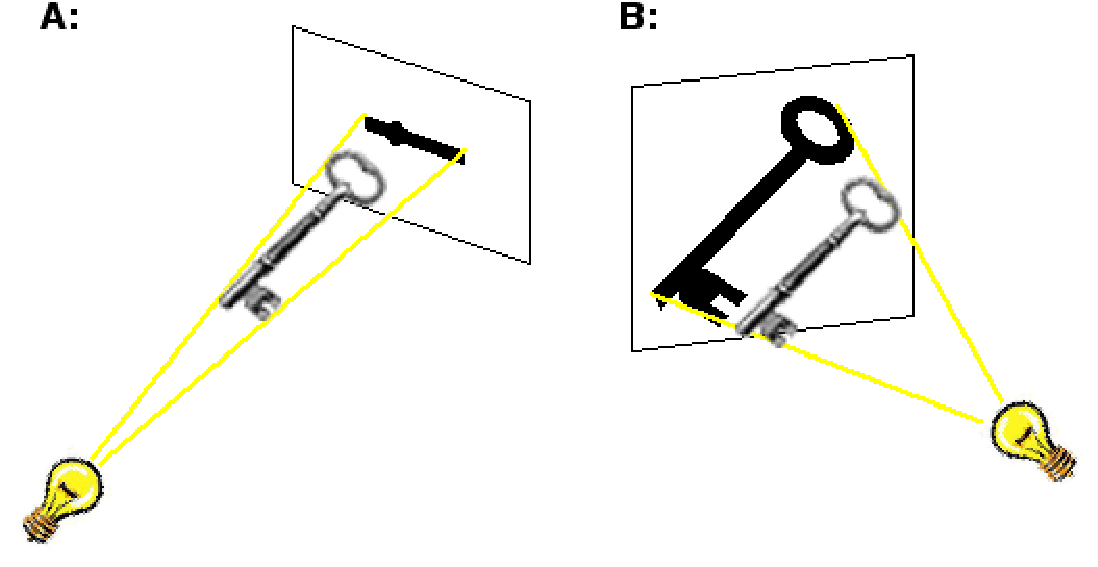
\includegraphics[height=.5\textheight,clip]{fig/projection2}
  \\ \black{A: minimum-variance projection; B: maximum variance projection}
 \end{center}
\end{uncoverenv}
\end{frame}

